\documentclass[russian, utf8, emptystyle]{eskdtext}
\usepackage{amsmath, amsthm, amssymb, amsfonts, footnote, titlesec, epstopdf, tabularx}
\newcolumntype{L}[1]{>{\raggedright\let\newline\\\arraybackslash\hspace{0pt}}m{#1}}
\newcolumntype{C}[1]{>{\centering\let\newline\\\arraybackslash\hspace{0pt}}m{#1}}   \newcolumntype{R}[1]{>{\raggedleft\let\newline\\\arraybackslash\hspace{0pt}}m{#1}}

\newcommand{\sectionbreak}{\clearpage}

\newcommand*\justify{%
	\fontdimen2\font=0.4em% interword space
	\fontdimen3\font=0.2em% interword stretch
	\fontdimen4\font=0.1em% interword shrink
	\fontdimen7\font=0.1em% extra space
	\hyphenchar\font=`\-% allowing hyphenation
}

%\let\oldsection\section

%\renewcommand{\section}{\pagebreak \oldsection}

\setlength{\footskip}{20pt}
\begin{document}
\thispagestyle{empty}

\begin{center}
	\ \vspace{-2cm}
	
	
\includegraphics[width=0.5\textwidth]{msu.eps}\\
	{\scshape Московский государственный университет \\ имени М.В.~Ломоносова}\\
	Факультет вычислительной математики и кибернетики\\
	Кафедра  автоматизации систем вычислительных комплексов
	
	\vspace{4cm}
	
	\textbf{{\Large Треско Константин Игоревич}}
	
	\vspace{1cm}
	
	{\Huge\bfseries
	Исследование и разработка средств многотемной классификации веб-страниц\\}
\end{center}

\vspace{1cm}

\center{{\normalsize ВЫПУСКНАЯ КВАЛИФИКАЦИОННАЯ РАБОТА}}

\vspace{2cm}

\vfill

\begin{flushright}
	\normalsize
	\textbf{Научные руководители:}\\
	к.ф.-м.н. М.И. Петровский\\
	Д.В. Царев
\end{flushright}

\vfill

\begin{center}
	Москва, 2015
\end{center}

\enlargethispage{4\baselineskip}


	
\newpage
\abstract{
	Целью данной работы является исследование и разработка системы сбора и многотемной классификации веб-страниц, с которыми работали пользователи, находящиеся внутри одной сети. Разрабатываемая система сбора должна удовлетворять требованиям масштабируемости (линейного роста расхода ресурсов при увеличении числа подключений) и защищености (пользователь не должен иметь возможности фальсифицировать собранные данные). Модуль классификации данных должен обеспечивать многотемную классификацию на основе машинного обучения с возможностью добавления и удаления тематик.\\
	В ходе работы был проведен обзор существующих средств многотемной классификации и средств реализации системы сбора. Также была реализована система сбора и многотемной классификации, удовлетворяющая поставленным выше требованиям, проведено тестирование, показавшее приемлемую масштабируемость.\\	
}
\section {Введение}

\subsection {Задача классификации}
Настоящая работа посвящена исследованию и разработке программных средств сбора и многотемной классификации текстовых данных веб-страниц. Задача классификации многотемных документов (multi-label classification), заключается в определении принадлежности документа к одному или нескольким классам (из предопределённого набора классов) на основании анализа совокупности признаков, характеризующих данный документ. В отличие от традиционной задачи классификации, классы могут пересекаться или быть вложенными, то есть документ может принадлежать нескольким классам. Классы, к которым принадлежит документ называются релевантными.
\begin{figure}[h]
	\begin{center}
		\includegraphics[width=14cm]{pic/ML_Classification.png}
		\caption{Многотемная и многоклассовая классификация}
		\label{fig:low_sigma}
	\end{center}
\end{figure}
\subsection {Области применения классификации веб-данных}
На сегодняшний день существует ряд задач, для решения которых требуются системы сбора и классификации контента, частным случаем которого является веб-контент:
\begin{itemize}
	\item {\bf Анализ работы сотрудников организации.}
	Определение тематик документов, с которыми работает пользователь. На основе полученной информации применение политик безопасности
	\item {\bf Фильтрации контента, для обнаружения информации, относящейся к определенному делу (eDiscovery\cite{eDiscovery}).}
	Документы и электронная почта могут фильтроваться в зависимости от присвоенных им классов, чтобы гарантировать, что только материалы с запрошенной бизнес-информацией в рамках расследуемого дела были найдены и сохранены.
	\item {\bf Определения конфиденциальности документа, для предотвращения утечек информации}
	По различным экспертным оценкам в настоящее время наибольшие риски для информационной безопасности представляют не внешние, а внутренние угрозы \cite{InfoWatch}
	Поэтому существует необходимость в средствах определения конфиденциальности документа
	
\end{itemize}

Далее будут рассмотрены классы индустриальных систем, функционал которых включает в себя классификацию текстовых данных (в том числе веб-данных), с которыми работают пользователи.
\begin{itemize}
	\item {\bf 	Системы управления корпоративным контентом (англ. Enterprise Content Management, ECM) } - программные решения для управления информационными ресурсами предприятия предоставляют программные средства сбора, анализа, управления, накопления, хранения и доставки документов в масштабах организации. В настоящее время большинство ECM систем включают в себя системы обнаружения данным, связанных с определенным судебным делом (англ. eDiscovery). Средства eDiscovery обеспечивают процесс, с помощью которого организации находят, получают, сохраняют и анализируют документы, связанные с делом.
	\item {\bf Системы предотвращения утечки данных (англ. Data Loss Prevention, DLP)} -
	программные решения для предотвращения утечек конфиденциальной информации и минимизации других рисков, связанных с внутренними угрозами.
\end{itemize}
\subsubsection{Основные методы сбора и классификации данных в корпоративных системах}
Поиск и анализ информации в ECM системах происходит следующим образом:
\begin{itemize}
	\item {\bf Сбор данных.} Системы сбора содержат компоненту, установленную на пользовательском компьютере и отвечающую за мониторинг деятельности пользователя. В терминологии IBM данные компоненты называются Искателями \cite{searcher}
	\item {\bf Применение методов анализа документов.} В терминологии IBM данный этап называется аналитическим конвейером \cite{analitic}.
	\item {\bf Индексация данных.} Компоненты индексации добавляют в индекс информацию о новых и измененных документах
	\cite{idx1,idx2,idx3}
\end{itemize}

Существуют три основных подхода к классификации данных в ECM системах
\begin{itemize}
	\item {\bf Классификация на основе обучающей выборки} (IBM Content Classification \cite{ContentClassification}, Symantec eDiscovery \cite{Symantec})
	\item {\bf Классификация на основе заданных правил}. Принадлежность документа к тому или иному классу определяется на основе эвристических правил (сигнатур). Правила могут формироваться на основе контекста – имя отправителя, директория создания и т.п., а также на основе контента – шаблоны текста, ключевые слова и т.п. 
	\item {\bf Определение категорий в неизвестных документах}.
	В задаче кластеризации нет предопределенного набора классов. Исходное множество документов разбивается на подмножество таким образом, чтобы документы в различных подмножествах существенно отличались.
\end{itemize}

В DLP системах выделяют следующие технологии классификации данных:
\begin{itemize}
	\item {\bf Цифровые отпечатки (англ. digital fingerprint)} - технология предназначена для защиты больших по объему документов, содержание которых не изменяется или меняется незначительно. Детектор цифровых отпечатков позволяет автоматически обнаруживать в анализируемом тексте цитаты из документов-образцов, содержащих конфиденциальную информацию.
	\item {\bf Анализ шаблонов} - технология предназначена для детектирования алфавитно-цифровых объектов по шаблону данных (маске) и позволяет наиболее эффективно выявлять факты пересылки персональных данных или финансовой информации. Кроме того, данная технология может использоваться как вспомогательный метод для обнаружения фактов несанкционированной пересылки внутренних документов, содержащих формализованные данные, образованные по определенному шаблону (например, договоров или счетов в случае детектирования банковских реквизитов, кодов классификаторов и т.д.).
	\item {\bf Машинное обучение} (InfoWatch \cite{bkf}, Symantec VML \cite{MachLearn}). Примерная схема работы классификатора такова: на вход подается обучающий набор документов, состоящий как из конфиденциальных так и не конфиденциальных документов. По этим наборам производится обучение и строится статистическая модель. Далее полученная модель используется для классификации неизвестным документов. При обнаружении конфиденциального документа производятся действия, предписанные политиками безопасности.
\end{itemize}

Основное преимущество машинного обучения заключается в том, что в отличие от других описанных технологий, оно предназначено для работы не со статическими, а с постоянно меняющимися документами.\\
\subsection{Специфика задачи классификации текстовых веб-данных}
Веб – страницы имеют следующие особенности
\begin{itemize}
	\item Содержимое веб-страниц не подлежит шаблонному разбору
	\item Содержимое имеет многотемную природу, то есть каждая  из страниц может одновременно принадлежать к нескольким тематикам
\end{itemize}
	\begin{figure}[h]
		\begin{center}
			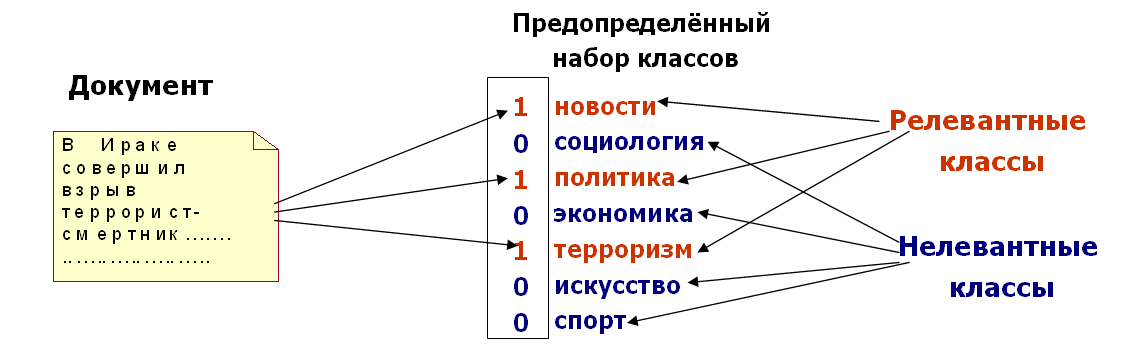
\includegraphics[width=14cm]{pic/Nature.png}
			\caption{Многотемная природа документа}
			\label{fig:low_sigma}
		\end{center}
	\end{figure}
\subsection{Выводы}
На сегодняшний день существует ряд прикладных задач, требующих классификации текстовых данных. Обзор индустриальных систем показал, что наиболее актуальными технологиями классификации текстовых данных являются:
\begin{itemize}
	\item Метод шаблонов
	\item Метод цифровых отпечатков
	\item Метод машинного обучения
\end{itemize}

Первые две технологии применимы только к статическим данным, в то время как метод машинного обучения позволяет позволять адаптироваться к тому, что содержимое и состав анализируемых данных постоянно меняется.\\
Для задачи классификации текстовых веб–данных из рассмотренных технологий подходит только машинное обучение с возможностью дообучения, так как веб – данные и набор классов постоянно меняются. \\
Рассмотренные системы решают задачу многоклассовой классификации, так как документ может принадлежать только к одному из предопределенного набора классу. Так как большая часть веб – данных имеет многотемную природу, то существует актуальность разработки системы сбора и многотемной классификации текстовых веб - данных пользователей. С учетом большого объема анализируемой информации к модулю классификации предъявляется требование масштабируемости. \\

Так как в рассмотренных системах присутствуют компоненты сбора информации, расположенные на пользовательских машинах, то при разработке системы сбора нужно учитывать то, что деятельность компонент никак не должна сказываться на работе пользователя, то есть к системе предъявляется требование производительности. Также в рассмотренных системах пользователь не имеет доступа к собираемой информации, поэтому система сбора должна удовлетворять требованию защищенности.
\section{Постановка задачи}
Разработать архитектуру и реализовать прототип системы сбора и многотемной классификации текстовых веб-данных пользователя в соответствии  с требованиями:
\begin{itemize}
	\item Модуль сбора должен обеспечивать
	\begin{itemize}
		\item Масштабируемость (линейный рост расхода ресурсов при росте числа подключений)
		\item Производительность (компоненты сбора, установленные на пользовательских машинах, не должны влиять на работу пользователя)
		\item Защищенность (пользователь не должен иметь возможности фальсифицировать данные)
		\item Функционирование под ОС Windows и браузером IE 
	\end{itemize}
	\item Модуль классификации должен обеспечивать
		\begin{itemize}
			\item Многотемную классификацию на основе машинного обучения с возможностью дообучения
		\end{itemize}
\end{itemize}
\section{Обзор}
Проведенный анализ систем ECM и DLP  в контексте задач классификации показывает, что каждый из пользователей является источником анализируемой информации, собираемая информация должна храниться в единой базе данных. Для управления потоком данных из различных источников используется мультиагентная система \cite{tan}. Под агентом подразумевается  автономный процесс, способный реагировать на среду исполнения и вызывать изменения в среде, возможно, в кооперации с пользователями или с другими агентами.\\
Разрабатываемая система должна состоять из:
\begin{itemize}
	\item Агентов мониторинга, расположенных на каждом из пользовательских компьютеров, собирающих текстовые данные просматриваемых пользователем веб – страниц и отправляющих их агенту консолидации
	\item Агента консолидации, принимающего данные от всех агентов мониторинга и сохраняющего их в единую базу данных
	\item Модуля классификации
\end{itemize}
Агент мониторинга состоит из двух компонент
\begin{itemize}
	\item Расширение для браузера, сохраняющее html код просматриваемой пользователем веб – страницы в локальную базу данных, расположенную на пользовательском компьютере
	\item Модуль передачи информации из базы данных агенту консолидации
\end{itemize}
\subsection{Расширение для браузера}
Для решения задачи необходимо расширение для браузера, имеющее возможность сохранить html код просматриваемой пользователем веб – страницы в локальную базу данных. Так как система сбора должна удовлетворять требованиям производительности, то сохранение и обработка данных должны происходить без участия пользователя.
\begin{itemize}
	\item {\bf BHO} (Browser Helper Object) - DLL-модуль, разработанный как плагин для Internet Explorer для обеспечения дополнительной функциональности. В BHO API существует возможность получения доступа к DOM текущей страницы. Также существует возможность обработки событий и управления навигацией. Для задачи перехвата контента данное решение подходит. Минусом является то, что данное решение подходит только для браузера IE. Но BHO имеет возможность записи и чтения данных из файловой системы пользователя, без его участия
	\item {\bf Kynext} позволяет перехватывать содержимое веб – страницы. Поддерживает IE, Firefox, Safari, and Chrome, но для написания необходимо использовать проприетарный язык Kynetx Rules Language. Еще одним минусом является то, что работа написанного расширение зависит от работоспособности самого расширения Kynext.
	\item {\bf WebMynd} поддерживает  IE, Firefox, Safari, and Chrome. Пока доступна бета версия, и не известно, будет ли дальнейшая поддержка продукта. Поддерживает JavaScript API. Не является бесплатным программным обеспечением.
	\item {\bf Crossrider} позволяет быстро создавать кросс-браузерные расширения. Использует один API и поддерживает JavaScript и jQuery, так что разработчик с базовыми знаниями JavaScript может писать и поддерживать свой код. Имеется возможность писать под IE, Firefox, Safari, and Chrome. Бесплатен в использовании. Существует документация и демо – видео для некоторых задач. Доступ к файловой системе пользователя только с его разрешения. 
\end{itemize}
\begin{table} 
	\caption{Средства расширения для браузера}
	\label{tab:far}
	\begin{center}
		\begin{tabular}{|L{5cm}|L{2cm}|L{2cm}|L{2cm}|L{2cm}|}
			\hline
			& BHO & Crossrider & Kynext & WebMynd \\
			\hline     
			Кроссплатформеность  & -(только IE) & + & + & + \\
			\hline
			Бесплатность & + & + & + & -\\
			\hline
			Поддерживаемые языки & C++,C\# & JavaScript & Kynext Rules Language & JavaScript  \\
			\hline
			Возможность записи в локальную ФС & + & - & - &- \\
			\hline
		\end{tabular}
	\end{center}
\end{table}
\subsubsection{Выводы из обзора средств реализации расширения браузера}

Компоненты системы сбора, установленные на пользовательских машинах не должны влиять на работу пользователя. Только BHO при сохранении файла не требует подтверждения пользователя. 

Таким образом для решения задачи сбора подходить только BHO, так как это средство может записывать в любое место на диске пользователя без его подтверждения.
\subsection{Методы многотемной классификации}
Можно выделить три основных подхода к многотемной классификации \cite{dis}
\begin{itemize}
	\item «Оптимизационный» подход 
	\item Подход на основе декомпозиции в набор независимых бинарных проблем 
	\item Подход на основе ранжирования
\end{itemize}
	\subsubsection{Методы, основанные на "оптимизационном"  подходе}
	К оптимизационным относятся методы классификации, в которых в явном виде задан показатель качества, который необходимо обратить в экстремум (максимум или минимум) по множеству допустимых разбиений.

	К данным алгоритмам можно отнести:
	\begin{itemize}
		\item Основанные на AdaBoost алгоритме (AdaBoost.MH \cite{AdaBoost},ADTBoost.MH \cite{ADT}) - минимизируется функция Hamming Loss)
		\item Multi-Label-kNN - \cite{kNN} максимизируются апостериорные вероятности принадлежности классам
	\end{itemize}

	Основной недостаток алгоритмов, основанных на оптимизационном подходе, заключается в том, что для решения задачи оптимизации необходимо хранение всего тренировочного набора, таким образом, нет возможности добавления и удаления тематик или дообучения
	\subsubsection{Методы, основанные на декомпозиции в набор независимых бинарных проблем}
	Кратко суть методов, основанных на декомпозиции в набор независимых бинарных проблем, можно описать так:
	\begin{itemize}
		\item Пусть дано N классов. Для каждого из N классов строится бинарный классификатор
		\item Далее, основываясь на решающей функции для каждого из классификаторов, можно определить релевантность класса
	\end{itemize}
	
Основным поводом для критики методов этой группы является то, что строятся независимые классификаторы, которые не учитывают корреляцию между классами, что существенно для многотемной классификации. Еще одним недостатком является высокая вычислительная сложность, так как количество бинарных подзадач равно числу классов, а каждая подзадача обучается на всём тренировочном наборе. 
\subsubsection{Методы, основанные на подходе ранжирования с последующим отсечением нерелевантных классов}
Работу алгоритмов можно разделить на два этапа
\begin{itemize}
	\item Первый этап состоит в обучении алгоритма ранжирования, который упорядочивает все классы по степени их релевантности для заданного классифицируемого объекта
	\item Второй этап заключается в построении функции многотемной классификации, отделяющей релевантные классы от нерелевантных
\end{itemize}
\subsection {Выводы из обзора методов многотемной классификации}
Обзор существующих методов классификации многотемных документов показал, что обозначенным в постановке задачи требованиям удовлетворяют только методы, основанные на подходе «каждый-против-остальных», но качество классификации не удовлетворяет потребностям прикладных задач. 

Поэтому был выбран алгоритм, разработанный в лаборатории Технологий Программирования, основанный на подходе попарных сравнений и удовлетворяющий всем поставленный требованиям.


\section {Исследование и построение решения}
\subsection{Разбиение на подзадачи}
Для решения задачи сбора и многотемной классификации текстовых данных веб – страниц пользователя был выбран мультиагентный подход \cite{multiagent}, поэтому система состоит из:
\begin{itemize}
		\item {\bf Агента мониторинга}, собирающего информацию и отправлющего ее агенту консолидации
		\item{\bf Агента консолидации}, сохраняющего информации со всех источников в единую базу данных
		\item{\bf Модуля классификации}, предоставляющего возможность определения принадлежности документа к одному из предопределенного набора классу
\end{itemize}
\subsubsection{Агент мониторинга}
\begin{figure}[h]
	\begin{center}
		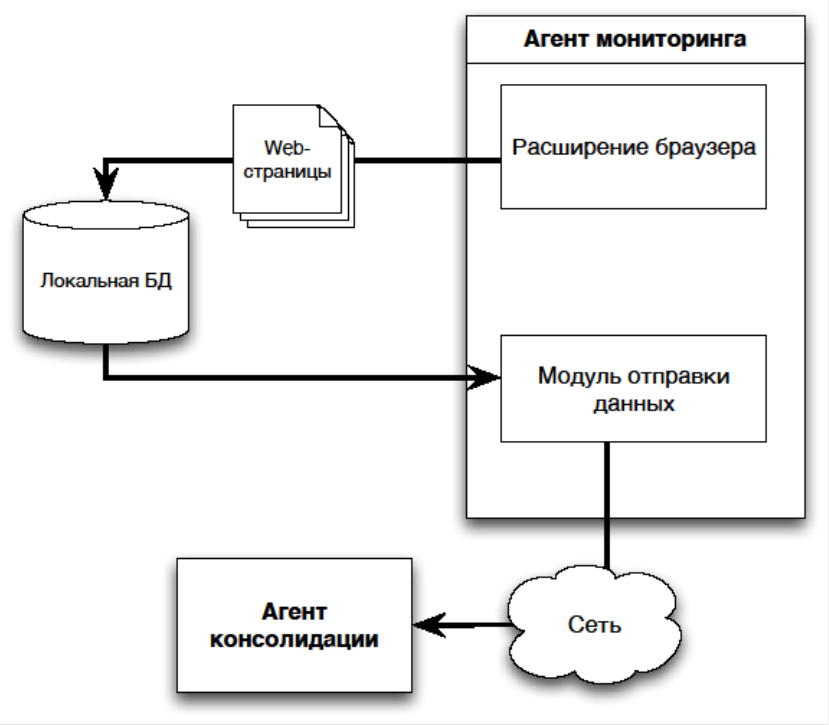
\includegraphics[width=10cm]{pic/agent1.png}
		\caption{Архитектура агента мониторинга}
		\label{fig:low_sigma}
	\end{center}
\end{figure}
Агент мониторинга состоит из нескольких компонент:
\begin{itemize}
	\item Расширение для браузера
	\item Модуль передачи данных агенту консолидации
\end{itemize}


Расширение для браузера, написанное с помощью BHO,  считывает html код просматриваемой пользователем веб-страницы и сохраняет ее в локальную базу данных. Сохранение в локальную базу данных осуществляется для контроля нагрузки на агент консолидации и возможности отправления данных по расписанию, а также на случай потери связи с агентом консолидации.

Модуль передачи данных агенту подключается к локальной базе данных и отправляет хранящуюся в ней информацию агенту консолидации, при получении ответа от агента консолидации отправленные данные удаляются из локальной базы данных, чтобы размер локальной базы данных не увеличивался постоянно.

Каждый из пользователей, является источником собираемой информации. При этом задача требует того, чтобы пользователь не имел доступа к собираемым данным. В случае реализации агента мониторинга с помощью BHO защищенность может осуществляться с помощью установки прав доступа на папку, в которой хранятся собираемые данные
\subsubsection {Агент консолидации}
\begin{figure}[h]
	\begin{center}
		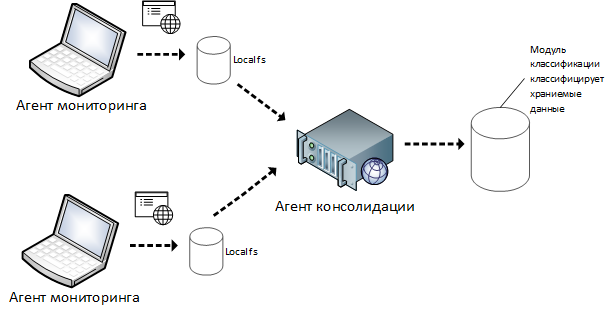
\includegraphics[width=14cm]{pic/agent2.png}
		\caption{Архитектура агента сбора}
		\label{fig:low_sigma}
	\end{center}
\end{figure}
Агент консолидации сохраняет данные, полученные от всех агентов мониторинга, в единую базу данных.Также в базу данных заносится дополнительная информация о страницах:
\begin{itemize}
	\item Логин пользователя, посещавшего веб-страницу
	\item Имя компьютера, на котором находится пользователь
	\item Дата посещения
	\item ID веб-страницы
\end{itemize}

При реализации необходимо учитывать то, что количество пользователей может быть достаточно велико, поэтому необходимо обеспечить приемлемую масштабируемость агента сбора
\subsubsection{Модуль классификации}
\begin{figure}[h]
	\begin{center}
		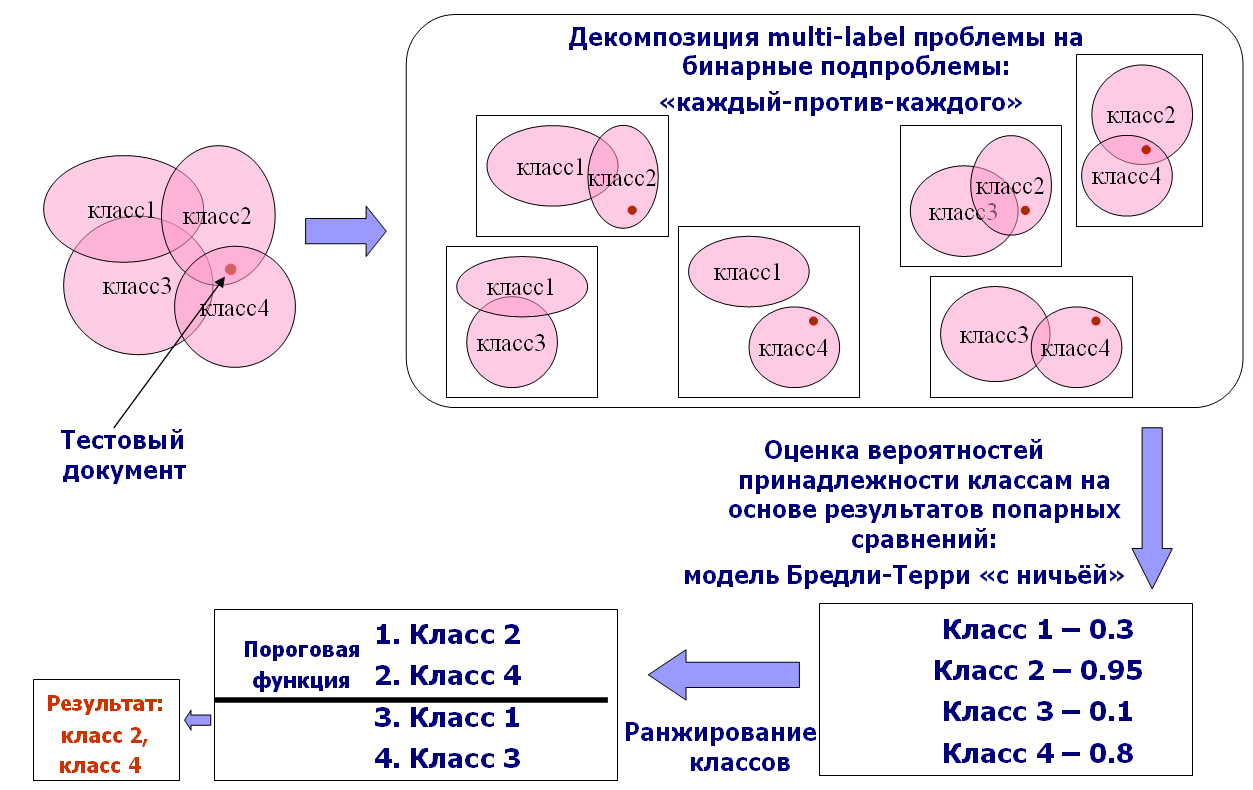
\includegraphics[width=14cm]{pic/module.png}
		\caption{Работа модуля классификации}
		\label{fig:low_sigma}
	\end{center}
\end{figure}
В ходе обзора было принято решение использовать модуль классификации, реализованный в лаборатории Технологий Программирования, основанный на подходе попарных сравнений (декомпозиция типа «каждый-против-каждого»). 

Предложенное решение включает новый алгоритм ранжирования, основанный на модифицированном для случая существенно пересекающихся классов, и новый алгоритм построения пороговой функции отсечения нерелевантных классов. 

Он предоставляет следующие сценарии работы:
\begin{itemize}
	\item {\bf Обучение.}Построение модели классификации на основе совокупности заранее рубрицированных гипертекстовых документов
	
	\item {\bf Классификация.}Применение построенной модели к новому классифицируемому документу
	\item {\bf Дообучение.}Модификация модели классификации на основе дообучения на новых документах с релевантными для них тематиками
	\item {\bf Удаление темы.}Удаление тематики классификации из модели без необходимости последующего обучения "с нуля"
\end{itemize}

\section{Описание практической части}
В данном разделе будет рассмотрена архитектура разработанного программного средства, представлен основной сценарий работы с ним, а также пояснены детали реализованных механизмов. Также будут приведены некоторые характеристики функционирования разработанного средства.
\subsection{Общая архитектура разработанного средства}
	\begin{figure}[h]
		\begin{center}
			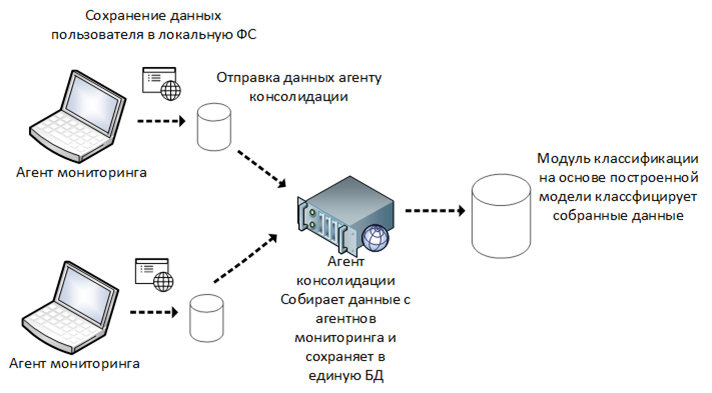
\includegraphics[width=12cm]{pic/arch.png}
			\caption{Архитектура прототипа}
			\label{fig:low_sigma}
		\end{center}
	\end{figure}
\subsubsection{Мониторинг пользователей}
Задача сбора просмотренных пользователем веб-страниц осуществляется с помощью расширения для браузера IE.

При открытии окна браузера расширение создает подключение к существующей базе данных, реализованных с помощью SQLite. Если нет базы данных нет, то создается новая, имеющая следующие поля:
\begin{itemize}
	\item Имя пользователя
	\item Имя компьютера
	\item URL просмотренной страницы
	\item Дата
	\item HTML код страницы
\end{itemize}

Каждый раз, когда пользователь загружает новую страницу, происходит событие, по которому html код просмотренной веб-страницы сохраняется в локальную базу данных.

Расширение написано с помощью BHO (Browser Helper Object) на языке программирования C\#, объем кода - 350 строк
\subsubsection{Сбор данных}

Каждый агент, расположенный на пользовательском компьютере подключается к базе данных, в которую были записаны данные расширением для браузера, и отправляет данные агенту сбора.

При настройке системы можно указать временной интервал, по которому будут отправляться данные. При отправке сохраняется время, когда была отправлена последняя просмотренная пользователем веб-страница.

При получении ответа от агента сбора, все записи, просмотренные до сохраненной временной метки удаляются, так как агент сбора успешно их сохранил, если же ответ не получен, то посылаются все записи, которые хранятся в базе.

Соединение агента мониторинга и агента сбора осуществляется с помощью TCP/IP сокетов. Каждый новый агент сбора обрабатывается в агенте консолидации асинхронно в отдельном потоке, что обеспечивает высокую скорость взаимодействия

Детали реализации модуля передачи данных агенту консолидации:
\begin{itemize}
	\item Количество строк кода - 250
	\item Язык реализации - C\#
	\item Доступ к локальной файловой системе без подтверждения пользователя осуществляется с помощью утилиты icacls \cite{icacls}, которая позволяет менять Integrity Levels \cite{icacls} файлов. Так как Internet Exploler имеет право записи только в папки с Low Integrity уровнем, то для записи в нужное место необходимо создать папку и указать Integrity Level. 
\end{itemize}

Агент сбора при получении посылает ответ агенту мониторинга, закрывает соединение и записывает полученные данные в единую базу данных, при этом к каждой записи добавляется ID.

Детали реализации агента консолидации:
\begin{itemize}
	\item Агент сбора был написан на примере асинхронного сокет сервера \cite{msdn}
	\item Язык написания - С\#
	\item Количество строк кода - 600
\end{itemize}
\subsubsection{Модуль многотемной классификации}
С учетом требований, сформулированных в постановке задачи, для многотемной классификации был выбран модуль, разработанный в лаборатории Технологий Программирования.

Для интеграции системы сбора с модулем многотемной классификации был написан модуль, который позволяет:
\begin{itemize}
\item Обучать классификатор, подавая ему на вход тренировочный набор, содержащий веб-страницу и тематику, к которой данный документ принадлежит
\item Выгружать веб-страницы из заданной базы данных и подавать их на вход классификатору. На выходе создается .csv файл следующего вида: 
\begin{table} [h]
	\caption{OutputeFile.csv}
	\label{tab:far}
	\begin{center}
		\begin{tabular}{|c|c|c|c|c|}
			\hline
			WebPageId & \(topic_1\) & \(topic_2\) & ... & \(topic_N\)  \\
			\hline     
			\(ID_1\)  & \(weight_{11}\) & \(weight_{12}\) & ... & \(weight_{1N}\) \\
			\hline
			\(ID_2\)  & \(weight_{21}\) & \(weight_{22}\) & ... & \(weight_{2N}\) \\
			\hline
			... & ... & .... & ... & .... \\
			\hline
			\(ID_N\)  & \(weight_{N1}\) & \(weight_{N2}\) & ... & \(weight_{NN}\) \\
			\hline
		\end{tabular}
	\end{center}
\end{table}
\end{itemize}
\subsection{Экспериментальные исследования}
В ходе обзора существующих решений было выдвинуто требование масштабируемости агента консолидации.

	
Так как разработка велась на языке программирования C\# в среде разработки Visual Studio, то для проведения нагрузочного тестирования было решено воспользоваться встроенными средствами Visual Studio \cite{test}.

Ход тестирования
\begin{itemize}
	\item Для нагрузочного тестирования были созданы Unit тесты \cite{unitTest}, содержащие код компоненты агента мониторинга, который взаимодействует с агентом консолидации
	\item Visual Studio позволяет выбирать такие параметры сценария тестирования как: начальное количество клиентов, максимально количество клиентов, и скорость увеличения
	количества клиентов
	\item Далее, задавая параметры сценариев, было проведено исследование зависимости нагрузки ЦП и оперативной памяти от количества подключенных клиентов
	 \begin{figure}[h]
	 	\begin{center}
	 		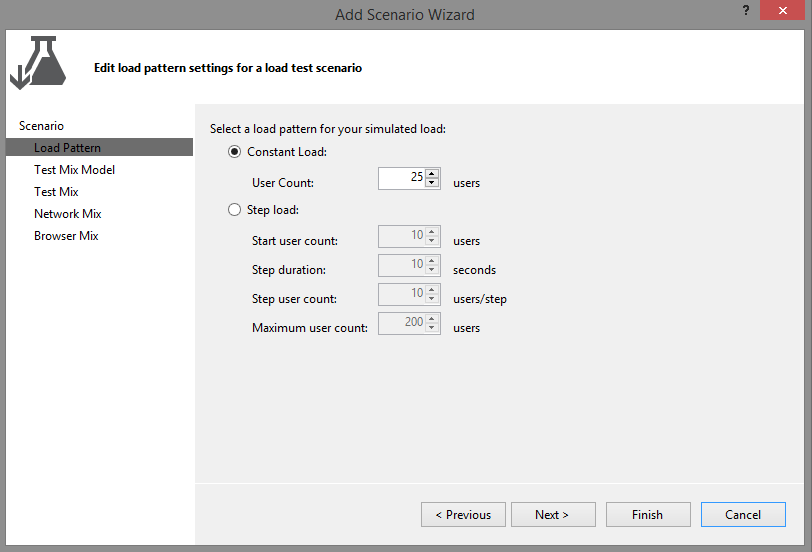
\includegraphics[width=14cm]{pic/test.png}
	 		\caption{Параметры сценария тестирования}
	 		\label{fig:low_sigma}
	 	\end{center}
	 \end{figure}
\end{itemize}
\subsubsection {Исследование зависимости нагрузки ЦП от количества подключенных клиентов}

Сценарий тестирования:
\begin{itemize}
	\item Начальное количество клиентов - 1. Каждый подключенный клиент с заданной частотой посылает агенту консолидации просмотренные пользователем веб-страниц
	\item С установленной скоростью увеличивается количество подключенных агентов мониторинга
	\item С помощью средств Visual Studio отрисовывается график, отражающий зависимость нагрузки ЦП от количества подключенных клиентов
\end{itemize}

Результаты тестирования проиллюстрированы ниже
 \begin{figure}[h]
 	\begin{center}
 		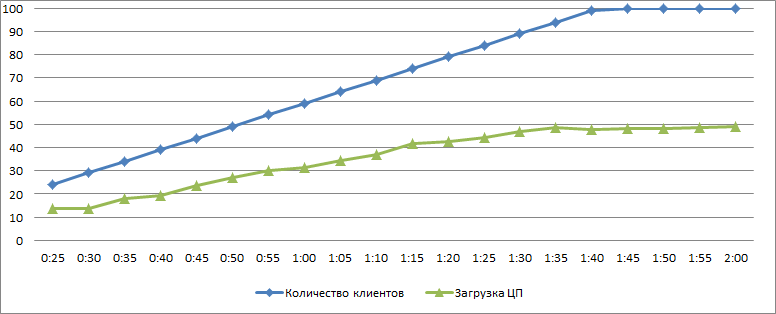
\includegraphics[width=12cm]{pic/test1.png}
 		\caption{Зависимость нагрузки ЦП от количетва клиентов}
 		\label{fig:low_sigma}
 	\end{center}
 \end{figure}
 
\subsubsection{Исследование использования оперативной памяти от количества клиентов}

Сценарий тестирования аналогичен сценарию из предыдущего пункта.
Результаты тестирования приведены ниже
\begin{figure}[h]
	\begin{center}
		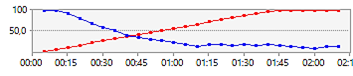
\includegraphics[width=12cm]{pic/test2.png}
		\caption{Зависимость использования оперативной памяти от количества клиентов}
		\label{fig:low_sigma}
	\end{center}
\end{figure}
\subsection{Итоги тестирования}

Зависимость нагрузки центрального процессора от количества подключенных клиентов линейна, что говорит о масштабируемости разработанного средства.

Увеличение использования оперативной памяти при увеличении количества подключенных клиентов достаточно линейно, что также говорит о масштабируемости разработанного средства
\section {Заключение}
В настоящей выпускной квалификационной работе были проведены исследования архитектур средств многотемной классификации веб-страниц.Был проведен анализ существующих алгоритмов многотемной классификации и выбран тот, который удовлетворяет требованиям поставленной задачи.

Была осуществлена программная реализация предложенной системы, состоящей из:
\begin{itemize}
	\item Агента мониторинга
	\item Агента консолидации
	\item Модуля многотемной классификации
\end{itemize}

Были разработаны сценарии и проведено нагрузочное тестирование, которое показало хорошую масштабируемость.

\begin{thebibliography}{50}
	\bibitem{InfoWatch}
	\textit {Аналитический Центр InfoWatch, Безопасность информации в корпоративных информационных системах. Внутренние угрозы}
	{(http://www.infowatch.ru/analytics/reports/4609)}
	\bibitem{ContentClassification}
	\textit {Component overview (Content Classification 8.8.0)}
	\bibitem{eDiscovery}
	\textit{Electronic discovery.}
	{(wikipedia.org/wiki/Electronic\_discovery)}
	\bibitem{Symantec}
	\textit {Предиктивное обучение}
	{(http://www.symantec.com/ru/ru/predictive-coding/)}
	\bibitem{bkf}
	\textit {Infowatch БКФ }
	{(http://www.infowatch.ru/technologies)}
	\bibitem {searcher}
	\textit{text}{122.	Component overview (IBM Watson Content Analytics 3.5.0)}
	{(http://www-01.ibm.com/support/knowledgecenter/SS5RWK\_3.5.0/com.ibm.discovery.es.nav.doc/iiysaovcomp.htm?lang=en)}
	\bibitem{analitic}
	\textit{Официальная документация IBM в Интернет}
	{(http://www-01.ibm.com/support/knowledgecenter/SS5RWK\_3.5.0/com.ibm.discovery.es.nav.doc/iiysaovcomp.htm?lang=en)}
	\bibitem{idx1}
	\textit{Content Analytics. Официальный сайт OpenText в Интернет}
	{(http://www.opentext.com/what-we-do/products/discovery/content-analytics)}
	\bibitem{idx2}
	\textit{EMC Kazeon File Intelligence}
	{(http://www.emc.com/content-management/emc-kazeon-file-intelligence.htm)}
	\bibitem{idx3}
	\textit{Using the Taxonomy Proposer to discover new categories}
	{(http://www-01.ibm.com/support/knowledgecenter/}
	\bibitem{MachLearn}
	\textit {Symantec Machine Learning}
	{(http://eval.symantec.com/mktginfo/enterprise/)}
	\bibitem{msdn}
	\textit{Асинхронный сокет сервер}
	{(https://msdn.microsoft.com/ru-ru/library/fx6588te(v=vs.110).aspx)}
	\bibitem{icacls}
	\textit{Утилита icacls}
	{(https://msdn.microsoft.com/en-us/library/bb625965.aspx)}
	\bibitem{unitTest}
	\textit{Create and run unit tests.}
	{(https://www.visualstudio.com/en-us/get-started/code/create-and-run-unit-tests-vs)}
	\bibitem{test}
	\textit{Walkthrough: Creating and Running a Load Test Containing Unit Tests}
	{(https://msdn.microsoft.com/en-us/library/vstudio/ff355993(v=vs.110).aspx)}
	\bibitem{tan}
	\textit{Таненбаум Э., Ван Стеен М.}
	{Распределенные системы. Принципы и парадигмы}
	\bibitem{AdaBoost}
	\textit{Schapire R. E., Singer Y. BoosTexter}
	{A boosting-based system for text categorization}
	\bibitem{ADT}
	{Comite F. D., Gilleron R., Tommasi M. Learning multi-label alternating decision tree from texts and data}
	{Machine Learning and Data Mining in Pattern Recognition, MLDM 2003 Proceedings, Lecture Notes in Computer Science 2734. Berlin, 2003. pp. 35–49s}
	\bibitem{kNN}
	\textit{Zhang M.-L., Zhou Z.-H. A k-nearest neighbor based algorithm for multi-label classification }
	{Proceedings of the 1st IEEE International Conference on Granular Computing (GrC'05). Beijing, China, 2005. pp. 718-721}
	\bibitem{dis}
	\textit{Глазкова В.В.}
	{Исследование и разработка методов построения программных средств классификации многотемных гипертекстовых документов}
\end{thebibliography}
\end{document}